% !TEX TS-program = pdflatex
% !TEX encoding = UTF-8 Unicode

% This file is a template using the "beamer" package to create slides for a talk or presentation
% - Introducing another speaker.
% - Talk length is about 2min.
% - Style is ornate.

% MODIFIED by Jonathan Kew, 2008-07-06
% The header comments and encoding in this file were modified for inclusion with TeXworks.
% The content is otherwise unchanged from the original distributed with the beamer package.

\documentclass{beamer}

\usetheme{AnnArbor}
\usecolortheme{wolverine}
\useoutertheme{shadow}
\useoutertheme{infolines}

\setbeamertemplate{headline}{}
\setbeamertemplate{footline}{}
\setbeamersize{text margin left=0.5cm}
  
\usepackage[english]{babel}
\usepackage{graphics, amssymb, pifont}
\usepackage[font = small]{caption}

\graphicspath{{../images/}{../graphs/}}

% Or whatever. Note that the encoding and the font should match. If T1
% does not look nice, try deleting the line with the fontenc.

\begin{document}

\title{Modeling the Deformation of a Golf Ball}
\subtitle{A Ball-Spring Simulation}
\author[Kar]{Kar Epker}
\date{April 12, 2012}
\institute{University of Michigan}

{
\setbeamertemplate{footline}{} 
\begin{frame}
\titlepage
\end{frame}
}
\addtocounter{framenumber}{2}

\begin{frame}{Introduction}

\begin{columns}

\column{0.5\textwidth}
\begin{itemize}
\item What is a force?
\item Deformations
\end{itemize}

\column{0.5\textwidth}
\begin{figure}
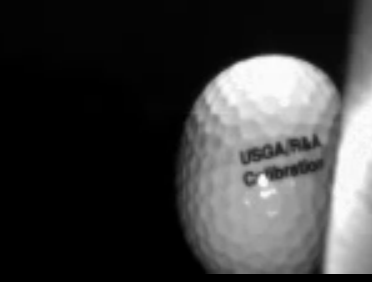
\includegraphics[width = 1.0\textwidth]{real_compression.png} \\
\scriptsize A United States Golf Association (USGA) video of a golf ball hitting steel at 150 mph
\end{figure}

\end{columns}
\end{frame}

\begin{frame}{Simulation}
\begin{columns}

\column{0.5\textwidth}
Two dif\mbox{f}iculties in simulating:
\begin{enumerate}[1.]
\item Making the model
\item Adding the physics
\end{enumerate}

\end{columns}
\end{frame}

\begin{frame}{Making the Model}
\begin{columns}

\column{0.5\textwidth}
\begin{itemize}
\item Geodesic spheres
\item Layers
\item Connections of particles
\end{itemize}

\column{0.5\textwidth}
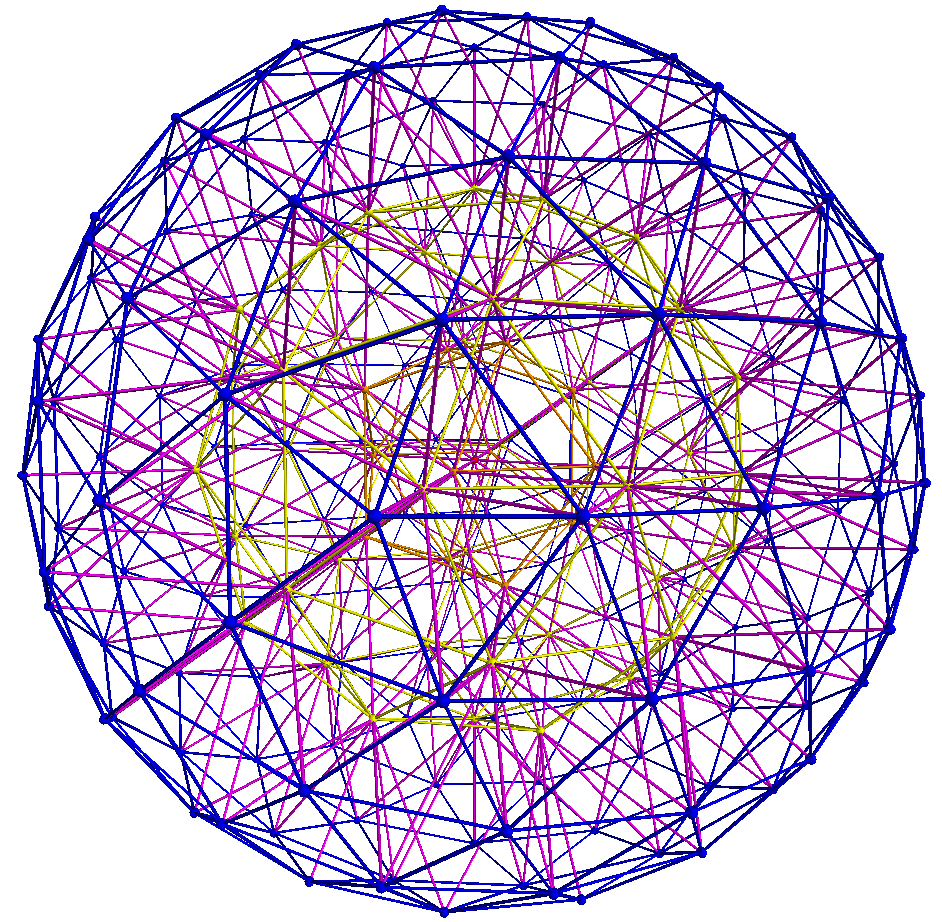
\includegraphics[width = 1.0\textwidth]{ball_spring_model.png}\\
\begin{center} \scriptsize The final model \end{center}

\end{columns}
\end{frame}

\begin{frame}{Adding the Physics}

\begin{itemize}
\item Springs
\item Revised momentum principle
\end{itemize}

\begin{columns}
\column{0.5\textwidth}
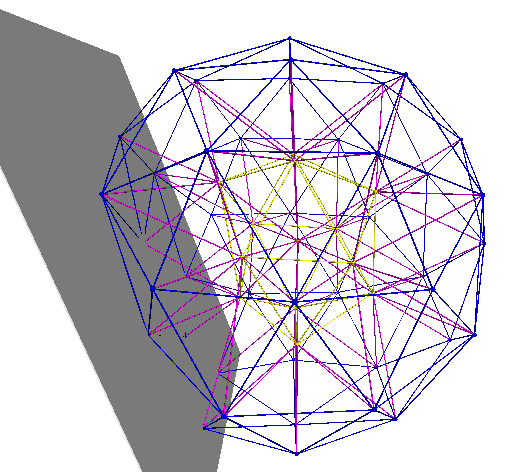
\includegraphics[width = 1.0\textwidth]{compression}
\begin{center}\scriptsize My model being compressed by a ``club'' \end{center}

\column{0.5\textwidth}
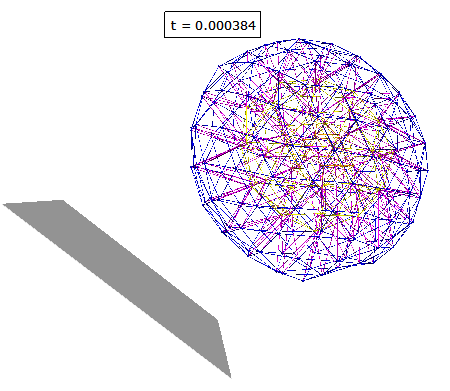
\includegraphics[width = 1.0\textwidth]{flying}
\begin{center}\scriptsize My model flying shortly after being hit \end{center}

\end{columns}
\end{frame}

\begin{frame}
\frametitle{Results}

Graphs of velocity of {\color{blue} edge getting hit}, {\color{yellow} the center of mass}, {\color{green} the dif\mbox{f}erence}

\begin{columns}
\column{0.33\textwidth}
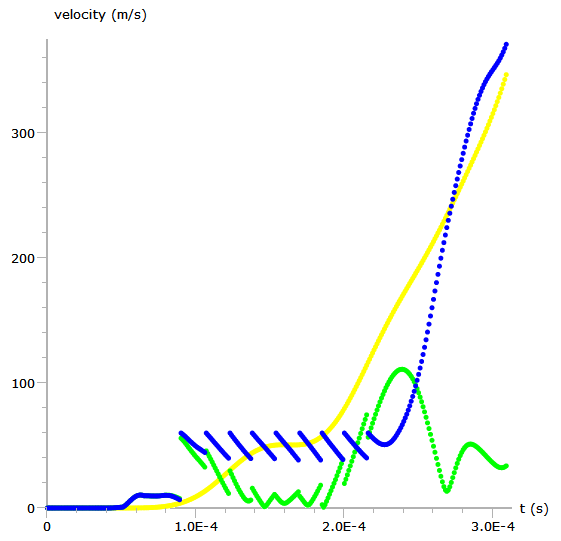
\includegraphics[width = 1.0\textwidth]{loft0}
\begin{center}\scriptsize Loft of $0^{\circ}$ \end{center}

\column{0.33\textwidth}
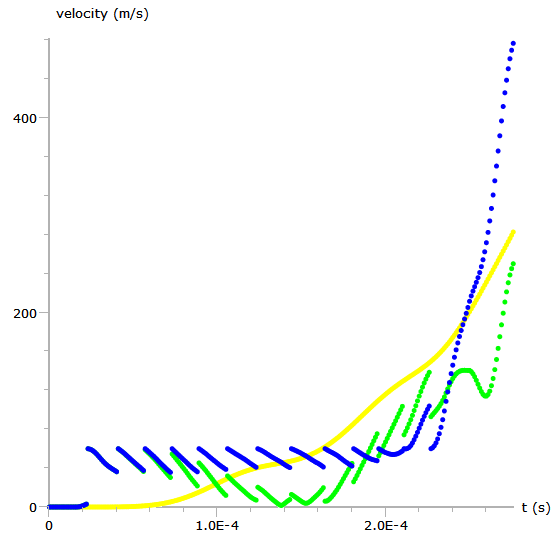
\includegraphics[width = 1.0\textwidth]{loft20}
\begin{center}\scriptsize Loft of $20^{\circ}$   \end{center}

\column{0.33\textwidth}
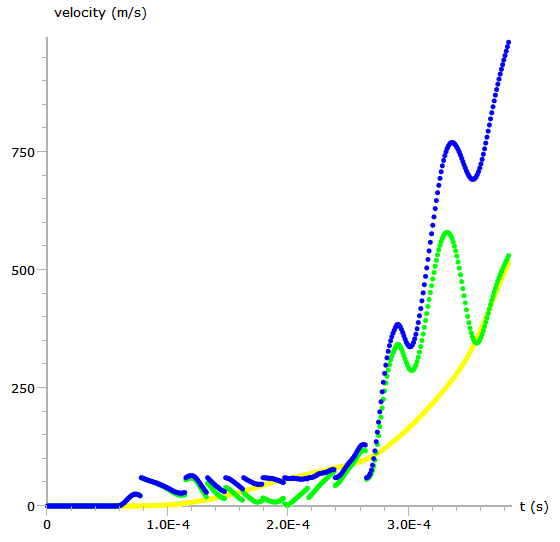
\includegraphics[width = 1.0\textwidth]{loft51}
\begin{center}\scriptsize Loft of $51^{\circ}$   \end{center}
\end{columns}

\pause

\begin{columns}
\column{0.5\textwidth}
\begin{center}The good parts:\end{center} \vspace{-2.5ex}
\begin{itemize}
\item Spin
\item Speed relative to each other
\end{itemize}
\pause

\column{0.5\textwidth}
\begin{center}The bad parts:\end{center} \vspace{-2.5ex}
\begin{itemize}
\item Speed quantitatively
\item Acceleration
\end{itemize}
\end{columns}

\end{frame}

\begin{frame}
\frametitle{Conclusions}
\begin{columns}

\column{0.5\textwidth}
\definecolor{amber}{RGB}{255, 126, 0}
\begin{description}
\item[{\color{green} \checkmark}] Deformation 
\item[{\color{green}\checkmark}] Spin
\pause 
\item[{\color{red}\ding{55}}] Verification/Validation
\item[{\color{red}\ding{55}}] Stability
\end{description}

\pause
\column{0.5\textwidth}
\begin{center}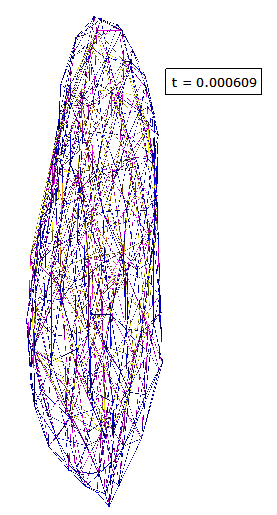
\includegraphics[height = 0.25\textheight]{flattening}\\
\scriptsize Flattening \end{center}

\begin{center}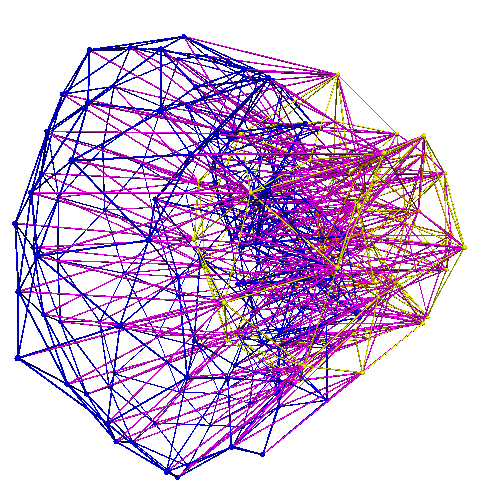
\includegraphics[width = 0.5\textwidth]{collapsing}\\
\scriptsize Collapsing \end{center}

\end{columns}

\pause
\begin{center}\vspace{2ex}The ultimate question: \textit{How do we debug nature?}\end{center}
\end{frame}

\end{document}


